\documentclass{article}

\usepackage[utf8]{inputenc}
\usepackage{graphicx}
\usepackage{latexsym}
\usepackage{listings}
\usepackage{mathtools}
\usepackage{textcomp}
\usepackage{float}
\usepackage{subfigure}

\title{COMP5400 Coursework2}
\author{Student ID: ml18p3h}
\date{\today}

\begin{document}

\maketitle

\section{Question 1}
Make a scatter plot of petal length against petal width. This means that for each entry in the data set you plot a point in the 2D plane with petal length as y coordinate, and petal width as x coordinate. Use three different markers (or different colours), one for setosa, one for versicolor and one for virginica. Plot other sepal/petal length/width combinations as well.
[10 marks]\\\\
\textbf{Answer:}\\
I use plot.py to make this scatter plot of petal length against petal width (the commented part of the code), as shown below.
\begin{figure}[H]
\centering
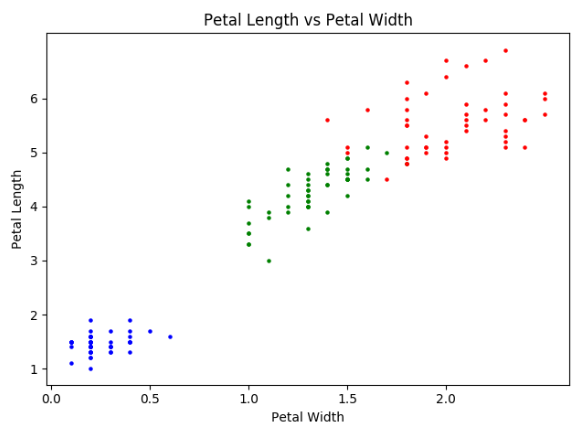
\includegraphics[scale=0.4]{./img/scatter.png}
\caption{petal length against petal width}
\end{figure}
\noindent
In addition, I draw a total plot including 16 subplots (12 subplots are useful actually), as shown below. They are the combinations of sepal/petal length/width, each parameter can be combined with three other parameters, that is why there are 12 useful subplots. It it note that the blue points represents setosa, the green represents versicolor, and red one means virginica.
\begin{figure}[H]
\centering
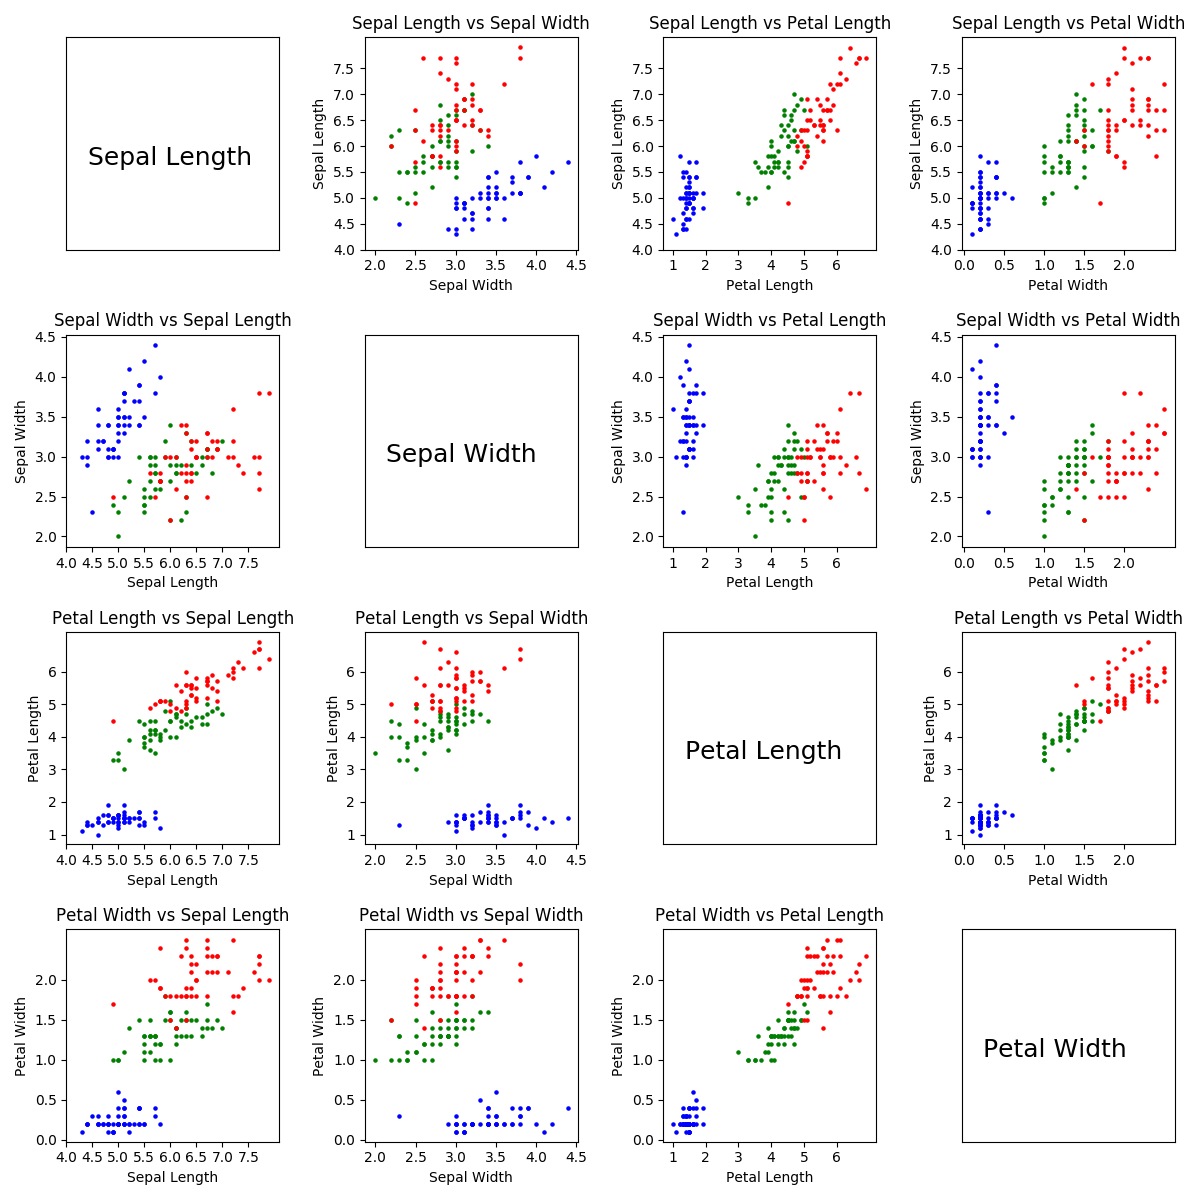
\includegraphics[scale=0.4]{./img/iris.png}
\caption{Iris Dataset (blue=setosa, green=versicolour, red=virginica)}
\end{figure}

\section{Question 2}
Based on the plots, do you believe that setosa vs. non-setosa can be learnt by a perceptron? That is, given a perceptron with 4 inputs, for petal length, petal width sepal length, and sepal width, can you find four weights and a bias which can classify setosa vs. non-setosa? Explain your answer. If you can, give these weights and bias. Draw the decision line of your perceptron on the plots of the last question.
[15 marks]\\\\
\textbf{Answer:}\\
From any of the 12 diagrams above, we can all draw a straight line separating the points of the setosa class from the colors of the other two classes. This shows that the setosa class is linearly separated from the non-setosa class. Thus it can be learned by the perceptron.\\
That setosa vs. non-setosa can even be classified by just two of these four features (petal length, petal width, sepal length and sepal width). There are many combinations of four weights and a bias which can classify setosa vs. non-setosa. For example, I choose the one in Q1, petal length against petal width. The figure including decision line of this perceptron as show below:\\
\begin{figure}[H]
\centering
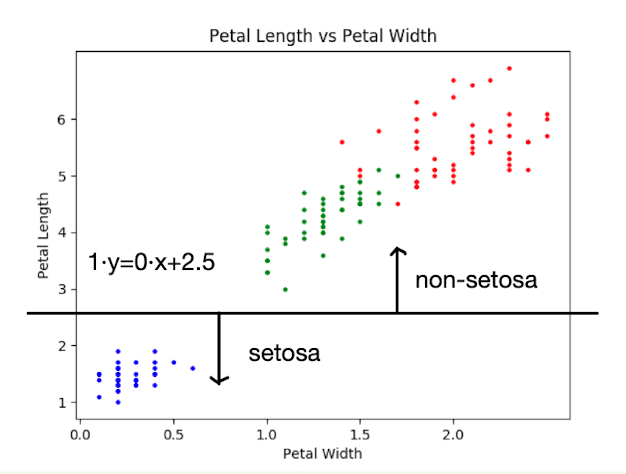
\includegraphics[scale=0.4]{./img/PLvsPW.png}
\caption{Petal Length vs. Petal Width}
\end{figure}
\noindent
In this figure above, a line $1*y-0*x-2.5=0$ separates setosa and non-setosa. The points below this line are classified as setosa and the points above this line are classified as non-setosa. This line $1*y-0*x-2.5=0$ can be replaced to $1*PL-0*PW-2.5=0$. Thus, from the parameters of this line, these four weights and a bias are $W_{sl}=0, W_{sw}=0, W_{pw}=0, W_{pl}=1, bias=-2.5$.

\section{Question 3}
Implement the standard perceptron algorithm without learning rate and train a perceptron for the setosa vs. non-setosa classification problem. Do you expect the algorithm to converge? Explain why! Does the algorithm converge? Is the output correct? If it does not converge, now introduce a learning rate, and use a sensible stopping criterion. Report the learning rate, stopping criterion and argue whether the result you obtain is in line with what you know the algorithm is capable of. The same questions about virginica vs. non-virginica? versicolor vs non-versicolor? There is a major difference between versicolor and the other two. Explain the difference using the plots you made.
[25 marks]\\\\
\textbf{Answer:}
\subsection{setosa vs. non-setosa}
I hope the algorithm to converge after training because it is easily to find a single decision line to separate the points of setosa and the points of non-setosa in each subplot in Figure 1 of Q1. From the result (as the figures shown below), we can conclude that the algorithm will converge and weights will not change frequently, with or without using learning rate.\\
With the learning rate 0.01, the accuracy after 150 epochs is nearly 87.33\% (usually between 80\% and 100\%), and the number of misclassified points is 19. The converge count is 91 means that weights are unchanged in 91 continuous epochs. Similarly, without using learning rate, the accuracy after 150 epochs is nearly 95.33\% and the number of misclassified points is only 7 and the converge count is 127. It can be said that this algorithm has converged.
\begin{figure}[H]
\centering
\subfigure[with learning rate 0.01]{
	\begin{minipage}[b]{0.46\textwidth}
	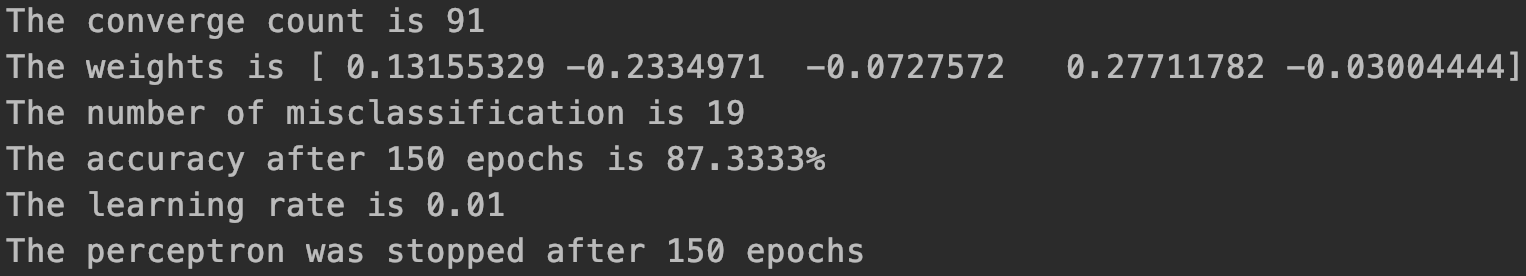
\includegraphics[width=1\textwidth]{./img/console1.png}
	\end{minipage}
}
\subfigure[without learning rate]{
	\begin{minipage}[b]{0.46\textwidth}
	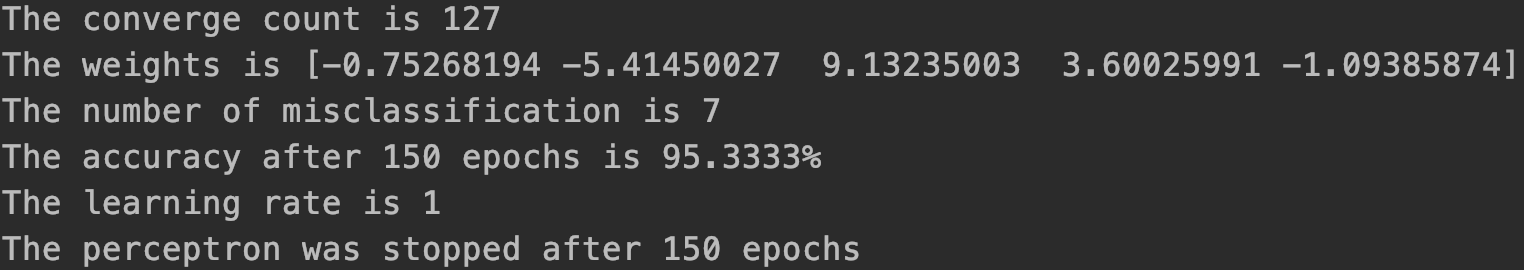
\includegraphics[width=1\textwidth]{./img/console2.png}
	\end{minipage}
}
\caption{result of separate setosa from non-setosa after 150 epochs} \label{fig:1}
\end{figure}
\noindent

\subsection{virginica vs. non-virginica}
As can be seen from the 12 subplots of Figure 1 in the Q1, the points of virginica partially overlap with the points of versicolor in each subplot, so that there is no decision line or decision boundary to separate all points of virginica from the points of non-virginica completely in these 2D subplots. Thus, virginica and non-virginica are not lineraly separable and the algorithm cannot converge completely.\\
By using a appropriate learning rate, the weights can be converged compared to without learning rate. The perceptron can find a hyperplane to separate the points of virginica and non-virginica nearly, as shown below. However, there still a few misclassified points on the margin of the part of virginica and non-virginica because there is no single hyperplace in the 4D to separate all points of virginica from the points of non-virginica actually.
\begin{figure}[H]
\centering
\subfigure[with learning rate 0.01]{
	\begin{minipage}[b]{0.46\textwidth}
	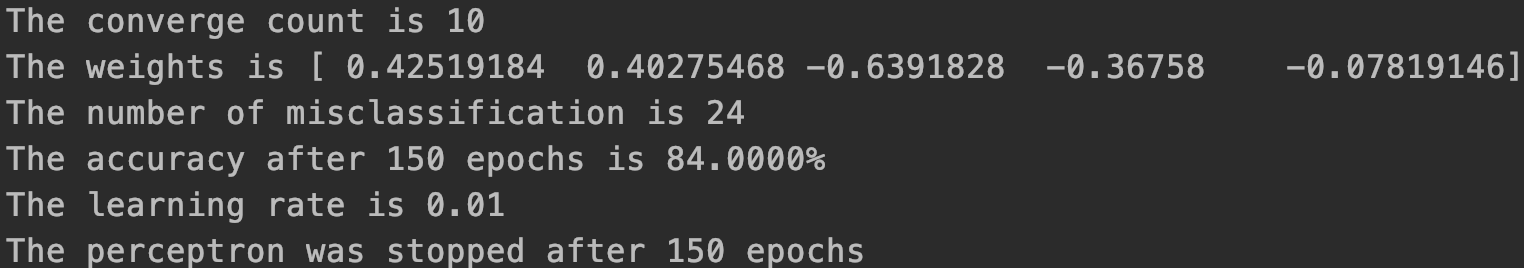
\includegraphics[width=1\textwidth]{./img/console4.png}
	\end{minipage}
}
\subfigure[without learning rate]{
	\begin{minipage}[b]{0.46\textwidth}
	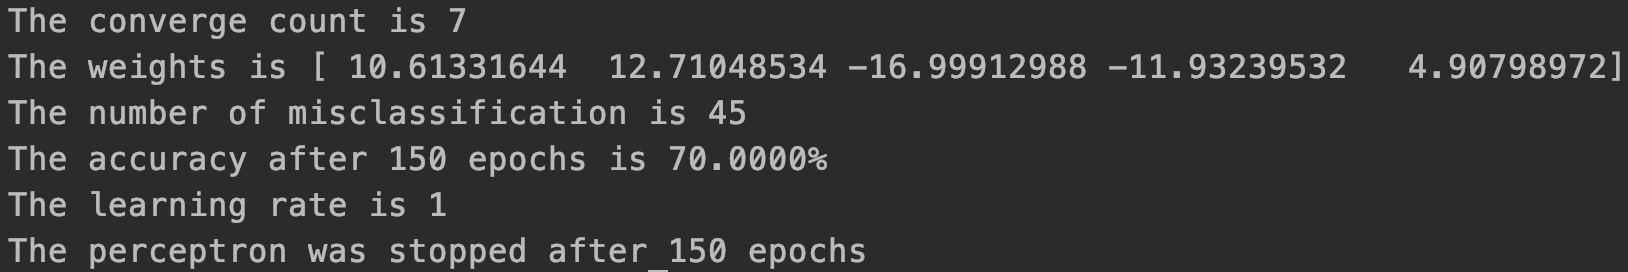
\includegraphics[width=1\textwidth]{./img/console3.png}
	\end{minipage}
}
\caption{result of separate virginica from non-virginica} \label{fig:1}
\end{figure}
\noindent

\subsection{versicolor vs. non-versicolor}                                                                                                                                                                                                                                                           
There is major difference between versicolor and the other two classes. Because as the Figure 1 shown above in Q1, the points of versicolor class lie between the points of the other two classes in each subplot. So, we cannot find just one decision line or decision boundary to almost separate the points of versicolor and non-versicolor, as shown below.\\
\begin{figure}[H]
\centering
\subfigure[with learning rate 0.01]{
	\begin{minipage}[b]{0.46\textwidth}
	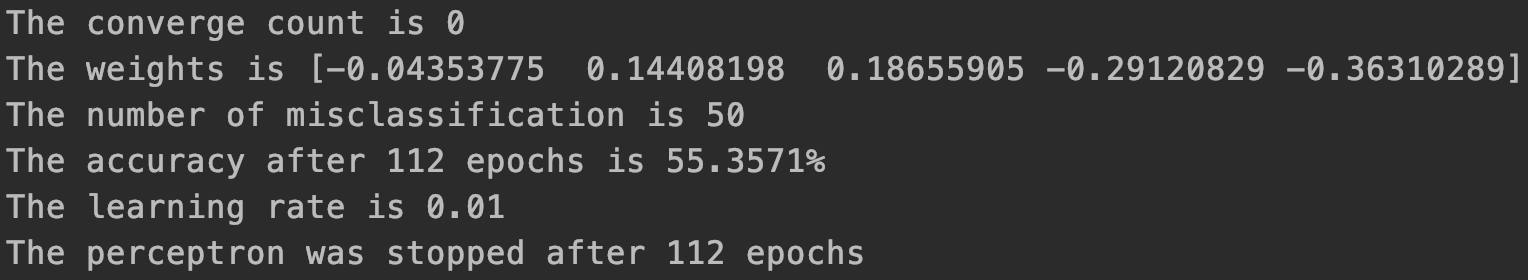
\includegraphics[width=1\textwidth]{./img/console6.png}
	\end{minipage}
}
\subfigure[without learning rate]{
	\begin{minipage}[b]{0.46\textwidth}
	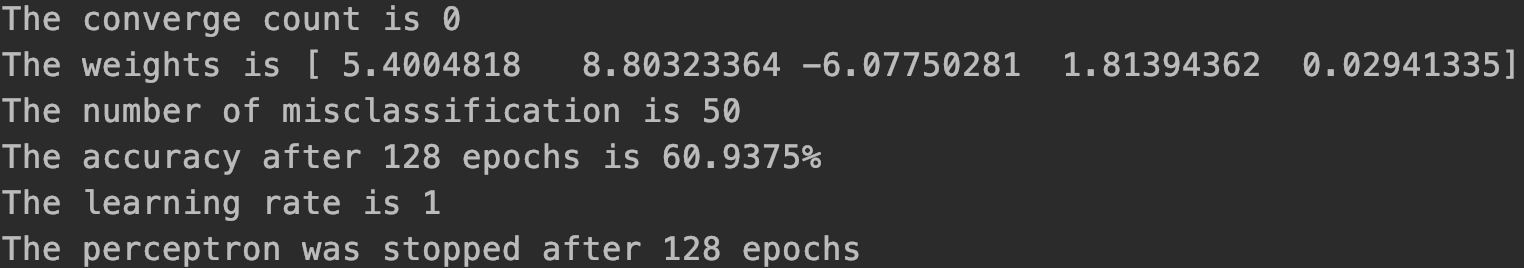
\includegraphics[width=1\textwidth]{./img/console5.png}
	\end{minipage}
}
\caption{result of separate versicolor from non-versicolor} \label{fig:1}
\end{figure}
\noindent
Hence, even we add learning rate to perceptron algorithm, the weights seem always change in each epoch which means that it cannot converge. The accuracy are between 49\% to no more than 65\%, and the number of misclassified points are always more than 50 (stopping criterion) when the training is not over.

\section{Question 4}
Using your earlier results, build a neural network with four inputs and three outputs. The network should produce the following desired classification: versicolor = (1,0,0), setosa = (0,1,0), virginica = (0,0,1). Do not use backpropagation. Combine the classifiers you have developed so far with some elementary logic - which you should implement using artificial neurons! Create a working program that implements your network. Your program must compile and run. Upon running, it must ask for 4 numbers: PL PW, SL, SW and produce a classification. In the report, explain the strategy you used, draw the full network and give all weights and biases. Evaluate the accuracy of your network.[20 marks]\\\\
\textbf{Answer:}\\
To build a neural network that produces the classification: versicolor = (1,0,0), setosa = (0,1,0), virginica = (0,0,1), we can combine the classifiers to build hidden layer. \\
\textbf{1.} At first, we can see that when the setosa and virginica output 0, the versicolor will output 1. This is a NOR gate. So, we can only use setosa and virginica to replace versicolor which means that there are only setosa and virginica neural in hidden layer without versicolor. Specifically, due to we define when output $\textless$ 0, it will output for 0 and when output $\geq$ 0, it will output for 1. Hence, for example, we can set setosa and virginica both output -1, and set bias to 0.5 to make balance to make virginica output 1 at the end. This a sub-neural network of versicolor as shown below. 
\begin{figure}[H]
\centering
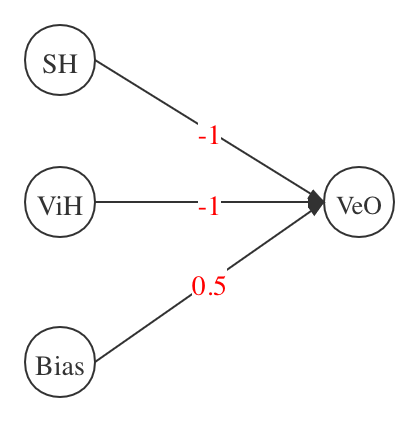
\includegraphics[scale=0.3]{./img/VeO.png}
\caption{versicolor neuron}
\end{figure}
\noindent
\begin{itemize}
	\item SH: setora perceptron in the hidden layer
	\item ViH: virginica perceptron in the hidden layer
	\item VeO: versicolor in the output layer
	\item SO: setosa in the output layer
	\item ViO: virginica in the output layer
	\item PL: petal length
	\item PW: petal width
	\item SL: sepal length
	\item SW: sepal width
	\item Bias: biases in the input layer and hidden layer
\end{itemize}
\textbf{2.} Then, it is clear that the setosa neural will output 1 if the perceptron of setosa inputs 1 so that it is a OR gate actually. In addition, due to we want to get setosa = (0,0,1), so we should make other elements to 0 which means we should set the weight of virginica to 0. To make balance, we set the value of bias to -0.5. The neural shows as following:
\begin{figure}[H]
\centering
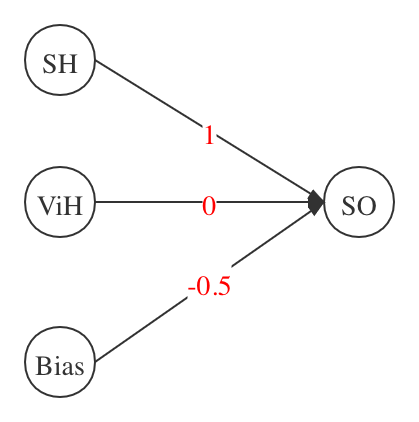
\includegraphics[scale=0.3]{./img/SO.png}
\caption{setosa neuron}
\end{figure}
\noindent
\textbf{3.} Next, the virginica is same as the setosa. Thus, we set the weight of virginica to 1, and weight of setosa to 0, and bias to -0.5. There is the neural network below:
\begin{figure}[H]
\centering
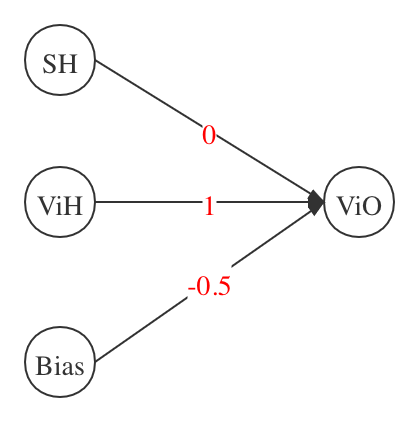
\includegraphics[scale=0.3]{./img/ViO.png}
\caption{virginica neuron}
\end{figure}
\noindent
\textbf{4.} The three outputs and hidden layer of the neural network have been built. Then, we should make 4 parameters: PL, PW, SL, SW as the input layer of this neural network. We use np.random.randn() to get 4 weights and a bias with standard normal distribution (the initialization resutls are different when we run it because it is random). Build the input layer by using these 4 weights and a bias as values for PL, PW, SL, SW and bias of input layer. The full neural network with all weights and biases as shown below:
\begin{figure}[H]
\centering
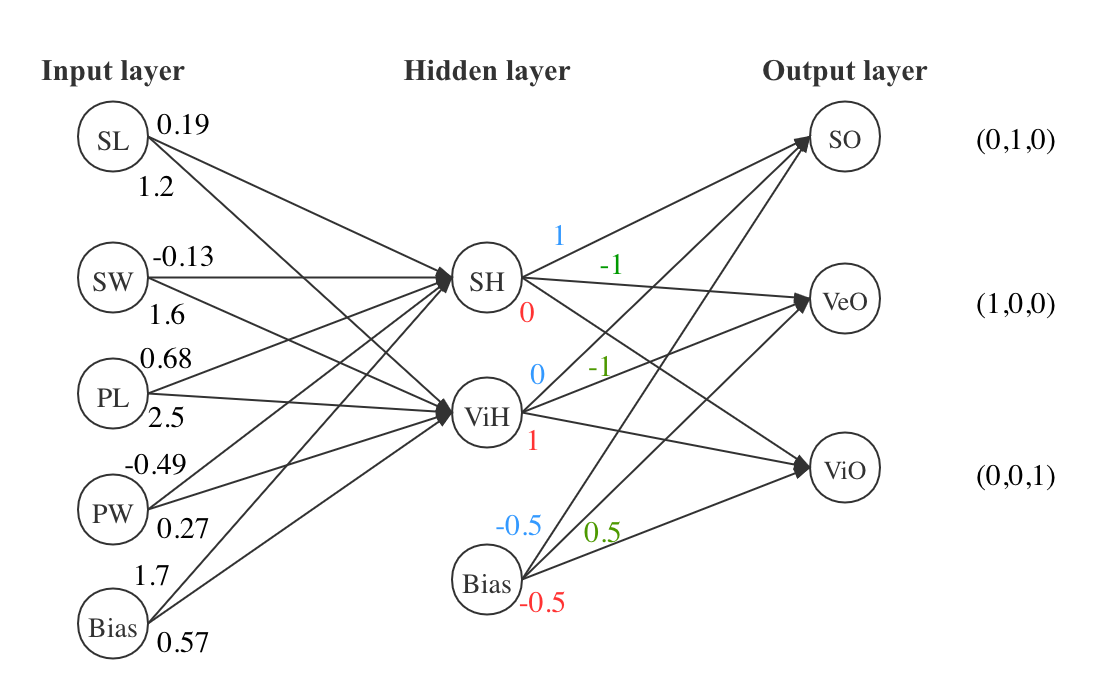
\includegraphics[scale=0.3]{./img/full_neural.png}
\caption{full network with all weights and biases}
\end{figure}
\noindent
Because the weights are initialized randomly each time, the accuracy of each run is also different. I decide to run 4 times and calculate an average of the accuracy as a result.
\begin{figure}[htbp]
\centering
\subfigure[accuracy1.]{
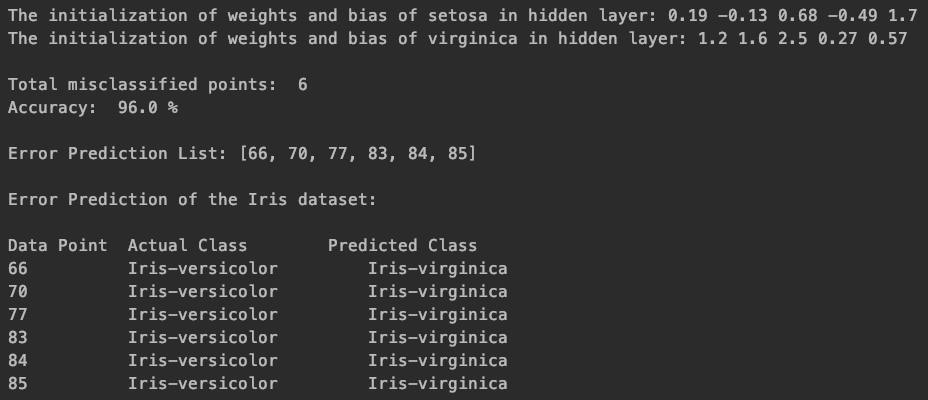
\includegraphics[width=5.5cm]{./img/accuracy1.png}
}
\quad
\subfigure[accuracy2.]{
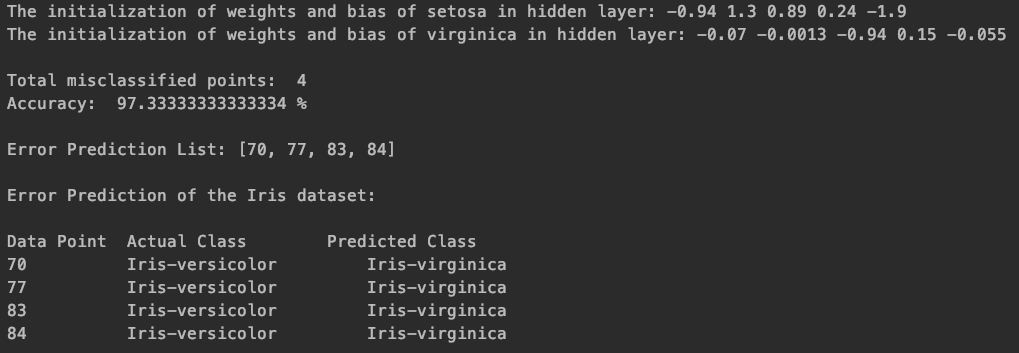
\includegraphics[width=5.5cm]{./img/accuracy2.png}
}
\quad
\subfigure[accuracy3.]{
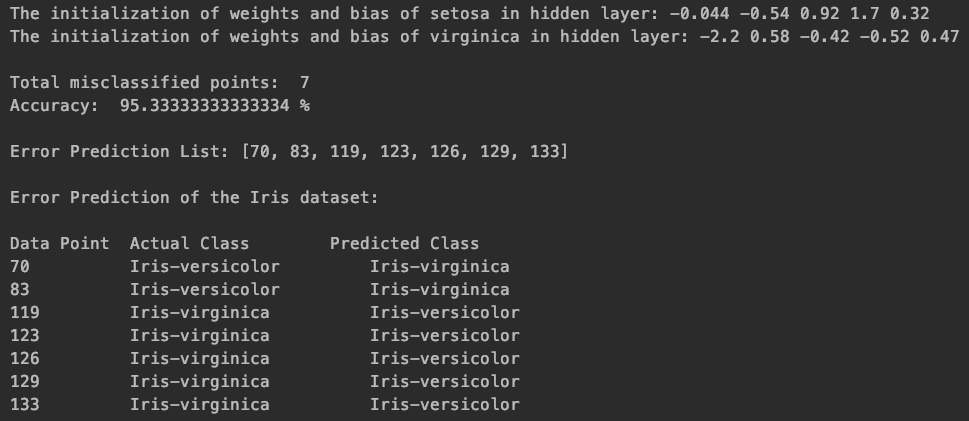
\includegraphics[width=5.5cm]{./img/accuracy3.png}
}
\quad
\subfigure[accuracy4.]{
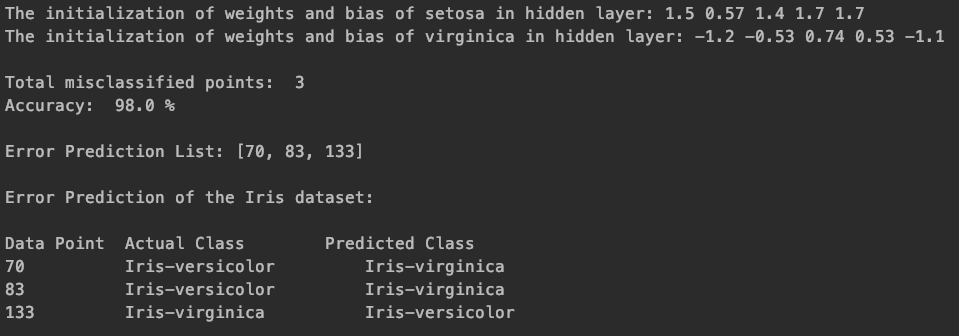
\includegraphics[width=5.5cm]{./img/accuracy4.png}
}
\caption{Accuracies}
\end{figure}
\noindent
The accuracies for the four runs are: 96.0\%, 97.3\%, 95.3\%, 98.0\%. Thus, the average of accuracies is 96.65\%, and as shown in the figure, there are an average of $(6+4+7+3) / 4 = 5$ misclassified points per run. The standard deviation is 1.0596\%.

\section{Question 5}
A tutorial will demonstrate an application of the Keras framework to solve the XOR problem. This implementation will be made available to you. You will then adapt this implementation for use on the iris data set.
Apply your implementation in a program that can classify the iris data. Create a demo program that can take 4 numbers PL PW, SL, SW and produce a classification. Evaluate the performance of your algorithm. Explain whether it is better or worse than the network you built in question 4. Give two reasons why your network cannot achieve perfect classification.
Experiment with the number of hidden nodes. Consider experimenting with the loss function. Make sure you create a training data set, and not to evaluate your network on this training data set.
[30 marks]\\\\
\textbf{Answer:}\\
Compared to AND or OR problems, XOR problem is inseparable (cannot find only one line to achieve linear separation), as shown below. However, perceptron is a linear classification model, so that single layer perceptron cannot solve XOR problem. We choose use the Keras framework to solve the XOR problem.
\begin{figure}[H]
\centering
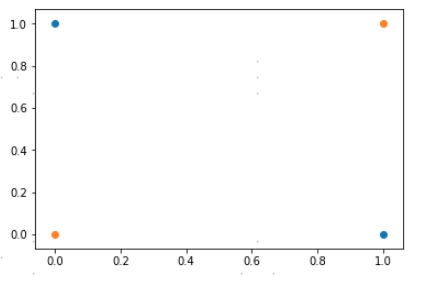
\includegraphics[scale=0.4]{./img/XOR.png}
\caption{XOR problem}
\end{figure}
\noindent
This model includes a hidden layer (4 nodes at first experiment) and an output layer (including 3 nodes which represent label predictionns). The input\_shape parameter of the input layer is correseponding to the number of features in this iris dataset, which means is 4.\\
We choose to use ReLU  for the hidden layer activation and softmax for the output layer activation. The optimization function of SGD with learning rate 0.01 and momentum 0.9. The full network model is as follows:
\begin{figure}[H]
	\centering
	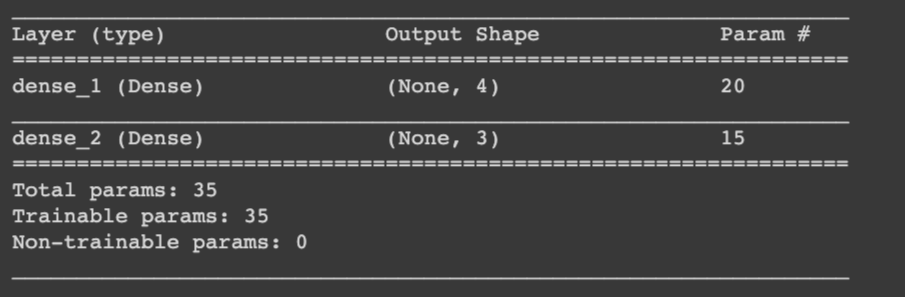
\includegraphics[scale=0.2]{./img/model.png}
	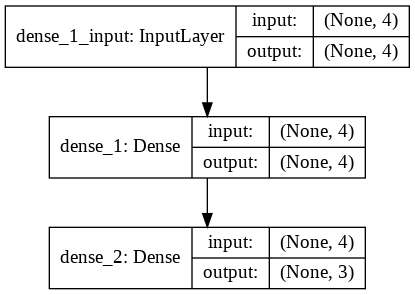
\includegraphics[scale=0.3]{./img/model_plot.png}
	\caption{full network model}
\end{figure}
\noindent
The loss and accuracy of last epoch is 5.32\% and 98.33\%, and the figure of loss and accuracy and confusion matrix are as shown below:

\begin{figure}[H]
\centering
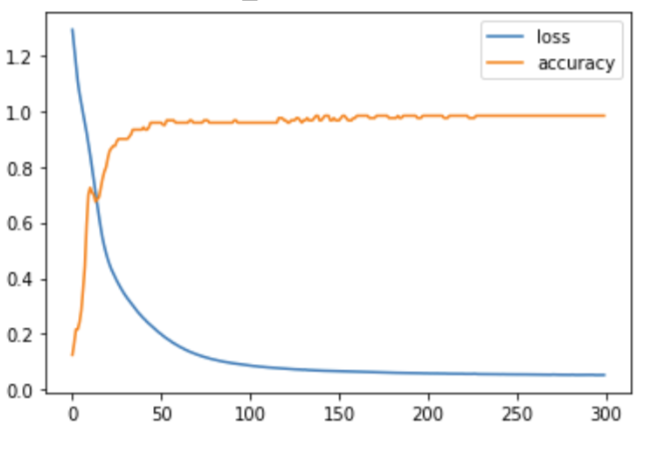
\includegraphics[scale=0.5]{./img/accuracy.png}
\caption{accuracy of Keras model}
\end{figure}

\begin{figure}[H]
\centering
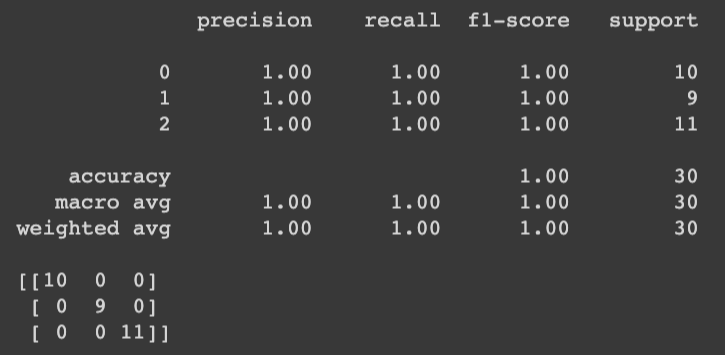
\includegraphics[scale=0.3]{./img/matrix.png}
\caption{connfusion matrix}
\end{figure}
\noindent
Due to the plot of loss and accuracy, it is clear to see that the curves have converged after 200 epochs. In addition, the accuracy is as high as 98\% (even more than 98\%), and the accuracy of the test data set (30 data) is 100\%, which means this algorithm or model by Keras is excellent.\\\\
It is clear that this model by Keras has better performace than the network I built in Q4. There are some reasons can explain why the network I built are not enough good:\\
\textbf{1.} At first, the network I built does not use backpropagation but Keras does. Keras uses the Dense layer to build the feedforward network to train with error reverse propagation algorithms. By using backpropagation, the neural network is constantly changing the connection weights of this network, so that the output of the network is constantly close to the desired output and error is reduced to the extent that it can be received.\\
\textbf{2.} Next, the network model I built uses gradient descent to update weights, however the model of Keras uses advanced activation, optimizer and loss function, which means it can update and compute network parameters that affect model training and model output to approximate to reach optimal values, thereby minimizing (or maxmizing) the loss function.\\\\
In addtion, I need to change the number of hidden nodes to consider experimenting with the loss function. The default number of nodes is 4. I change it to 10 and 100, retrain the model and get the figure of loss and accuracy, as shown below:

\section{Instruction and Usage}
This is the instruction and usage of this coursework. This compressed file contains the source code and resources as follows:
\begin{itemize}
	\item transfer.py: transfer Iris.data to Iris.csv, add header into file
	\item plot.py: a scatter plot of sepal/petal length/width combinations of Q1
	\item perceptron.py: implement a percetron to train setosa vs. non-setosa, virginica vs. non-virginica and versicolor vs. non-versicolor of Q3
	\item network.py: a full network model of Q4
	\item Keras\_Iris.ipynb: a network built by Keras of Q5
	\item img folder: including the generated images
	\item data folder: including the the data of Iris data set
\end{itemize}
Specifically, if we want to run perceptron.py, we can open the terminal and type in the following type:
\begin{center}
python perceptron.py $\textless$class$\textgreater$ with
\end{center}
The $\textless$class$\textgreater$ can be reaplced by the name of class, like setosa, virginica and versicolor. Also, `with' means with learning rate 0.01, `without' means without using learning rate. For example:
\begin{center}
python perceptron.py setosa without
\end{center}
As for Keras\_Iris.ipynb, we are supposed to run it via Juypter Notebook or Google Colab.\\
In addition, this .tar file also includes a PDF report and .tex, a LaTex source file.
\end{document}